\chapter{STUDY II - BACK SIDE DIAGNOSIS}\label{chp:Back Side Diagnosis}

In this chapter, an overview of the new pre-diagnosis (i.e., side) will be discussed—this system is based on Achilles tendonitis. Accordingly, general system analysis and design decisions will be addressed in Section \ref{sec:StudyIIAnalysisAndDesign}. Then, Section \ref{sec:StudyIIImplementation} delves into the specifics of implementation. Finally, in Section \ref{sec:StudyIITestAndEvaluation}, the initial test results and evaluation phase will be discussed.

\section{ANALYSIS AND DESIGN} \label{sec:StudyIIAnalysisAndDesign}

The primary system focus will not be changed, which is discussed in Chapter \ref{chp:Foot Detection & Primary Diagnosis}. However, this chapter profoundly focuses on the changes made to the system. Therefore, changes in requirements and design decisions will be discussed in this section.

As discussed in Section \ref{sec:StudyITestAndEvaluation}, a lack of supervision causes data to be unusable and unstable test environments. Therefore, the system should be used by healthcare officials or supervised.

\begin{figure}[htbp]
\centering
\fbox{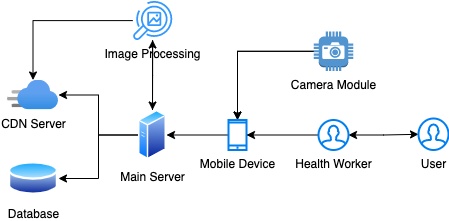
\includegraphics[width=.6\columnwidth]{KaanEksenMSc/figures/SystemOverviewStudyII.png}}
\caption{Architecture diagram of the updated system}
\label{fig:GeneralArchitectureDiagramPartI}
\end{figure}

In addition, based on the remote image evaluations, there may be conflicting results based on the index usage, which is discussed in Section \ref{sec:StudyITestAndEvaluation}. Therefore, physicians' diagnosis results should be added after examinations to assess the diagnosis correctly. The general structure of the converted system can be seen in Figure \ref{fig:GeneralArchitectureDiagramPartI}. 

\subsection{ PREDICTION AND FINE TUNE MODULE }

The prediction module is consists of the end-user interactions and pre-diagnosis. However, for improving results and more accurate testing, pre-diagnosis should be disabled since healthcare professionals will guide the participants. On the other hand, fine-tune module is consists of background procedures and healthcare professionals' interactions. Likewise, healthcare interaction modules will not be used since all diagnoses should be produced on examination. In the following paragraphs, details of the changes will be discussed.

End-user interactions on prediction module should be updated to usable by the healthcare professionals for supervised data collection. Same application flow should be protected except for the minor modifications such as healthcare professionals should be able to enter the diagnosis of the patients.

In the requirement analysis, discussions were conducted with the health professionals where they expressed the importance of Achilles tendonitis in the diagnosis process. Therefore, the automated index calculation process should be based on the achilles tendon to pre-diagnosis more accurately.

\subsection{ INDEX CALCULATION }

The pre-diagnosis, the system's underlying structure, which reduces the workload of healthcare professionals, should be updated to improve the results. Based on the importance of the Achilles tendon, the rearfoot angle is the best index calculation method for this calculation. 

Therefore, photographs of the back of the foot should be taken, and the rearfoot angle calculations should be made. These photos must include the calf and up to the foot's heel. In addition, legs should be centered for more accurate calculations.

\section{IMPLEMENTATION}\label{sec:StudyIIImplementation}

Implementation details of the changed modules will be discussed in this section. A more detailed explanation is provided by dividing it into subsections. 

\subsection{END-USER APPLICATION}

There were no significant changes in the en user application, but minor changes were made to improve the usability. Since users are not directly using the application, some user identification options are removed, such as phone numbers. In addition, some of the optional fields for students are also removed (see Figure \ref{fig:UserApplicationStudyIChanges}).

\begin{figure}[htbp]
\centering
\fbox{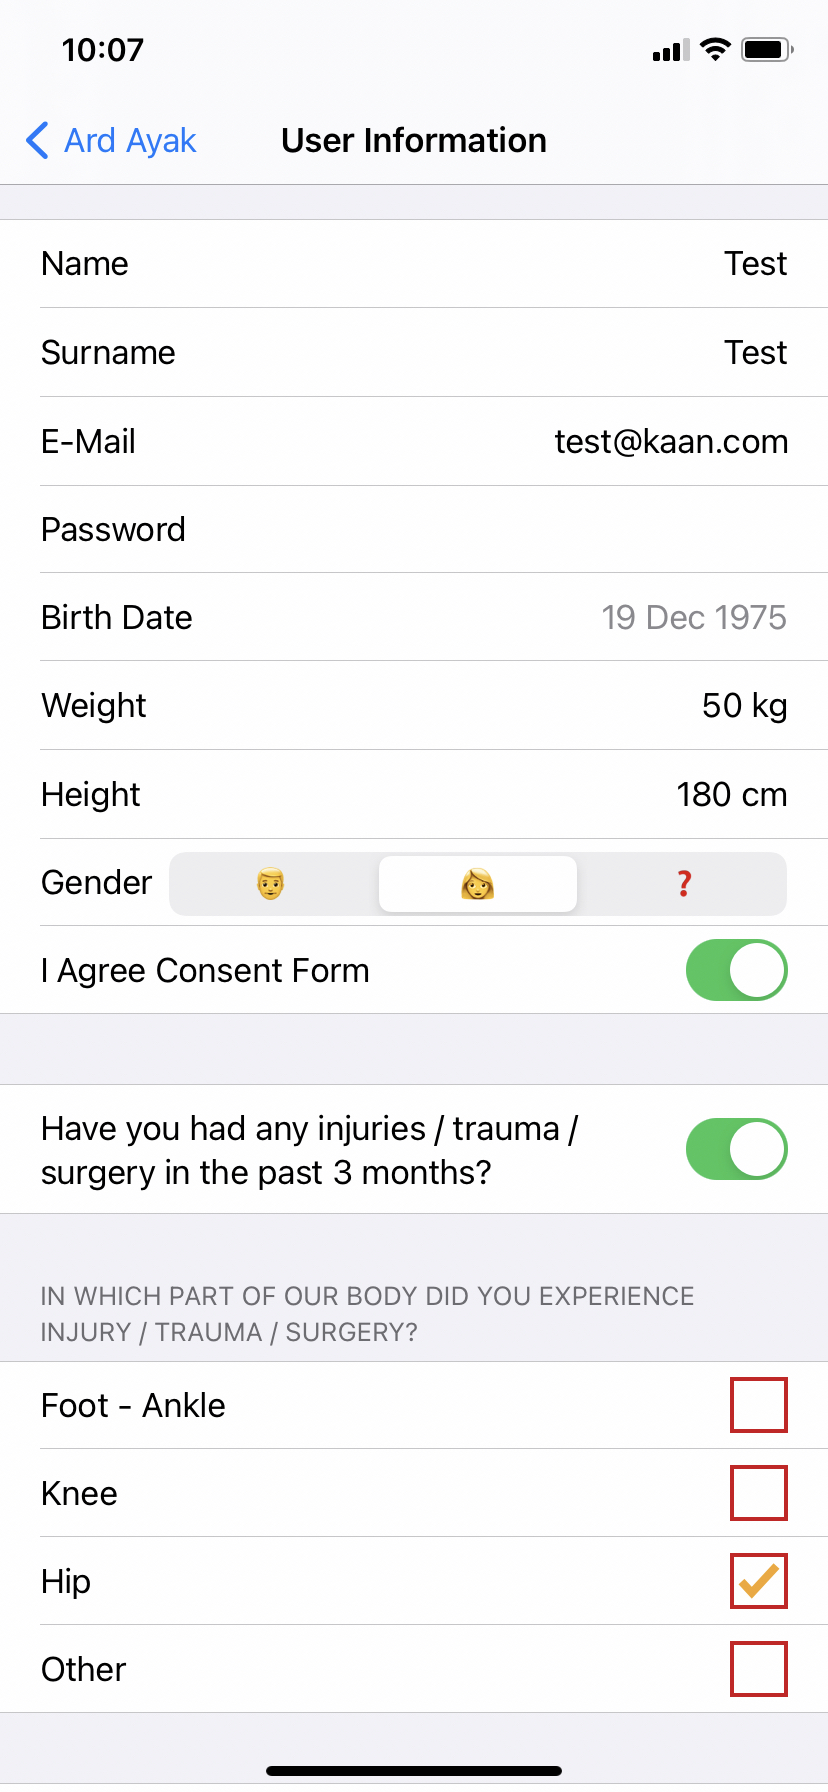
\includegraphics[width=.41\columnwidth]{KaanEksenMSc/figures/UserApplicationStudyIChanges.jpeg}}
\caption{Minor changes in end-user application in study I}
\label{fig:UserApplicationStudyIChanges}
\end{figure}

In addition to compliance with the needs requirement analysis, some minor errors have been fixed such as default values and crashes. Furthermore, the diagnostic results were collected as if the doctors entered them, not as if they were taken from the patient.

\subsection{SERVICES AND BATCH PROCESS}

Except for minor adjustments and bug fixes, no significant changes in services have been made. Most of the changes were conducted in the batch process for different index calculations in the automated process. Therefore in this subsection, all the changes will be discussed. 

One of the most significant service adjustments is made in the API. Diagnosis by option is added, which were recorded in different fields in the database (see Section \ref{sec:StudyIDatabase} for details). In addition, user type control is added to prevent misconfiguration.

\begin{figure}[htbp]
\centering
\fbox{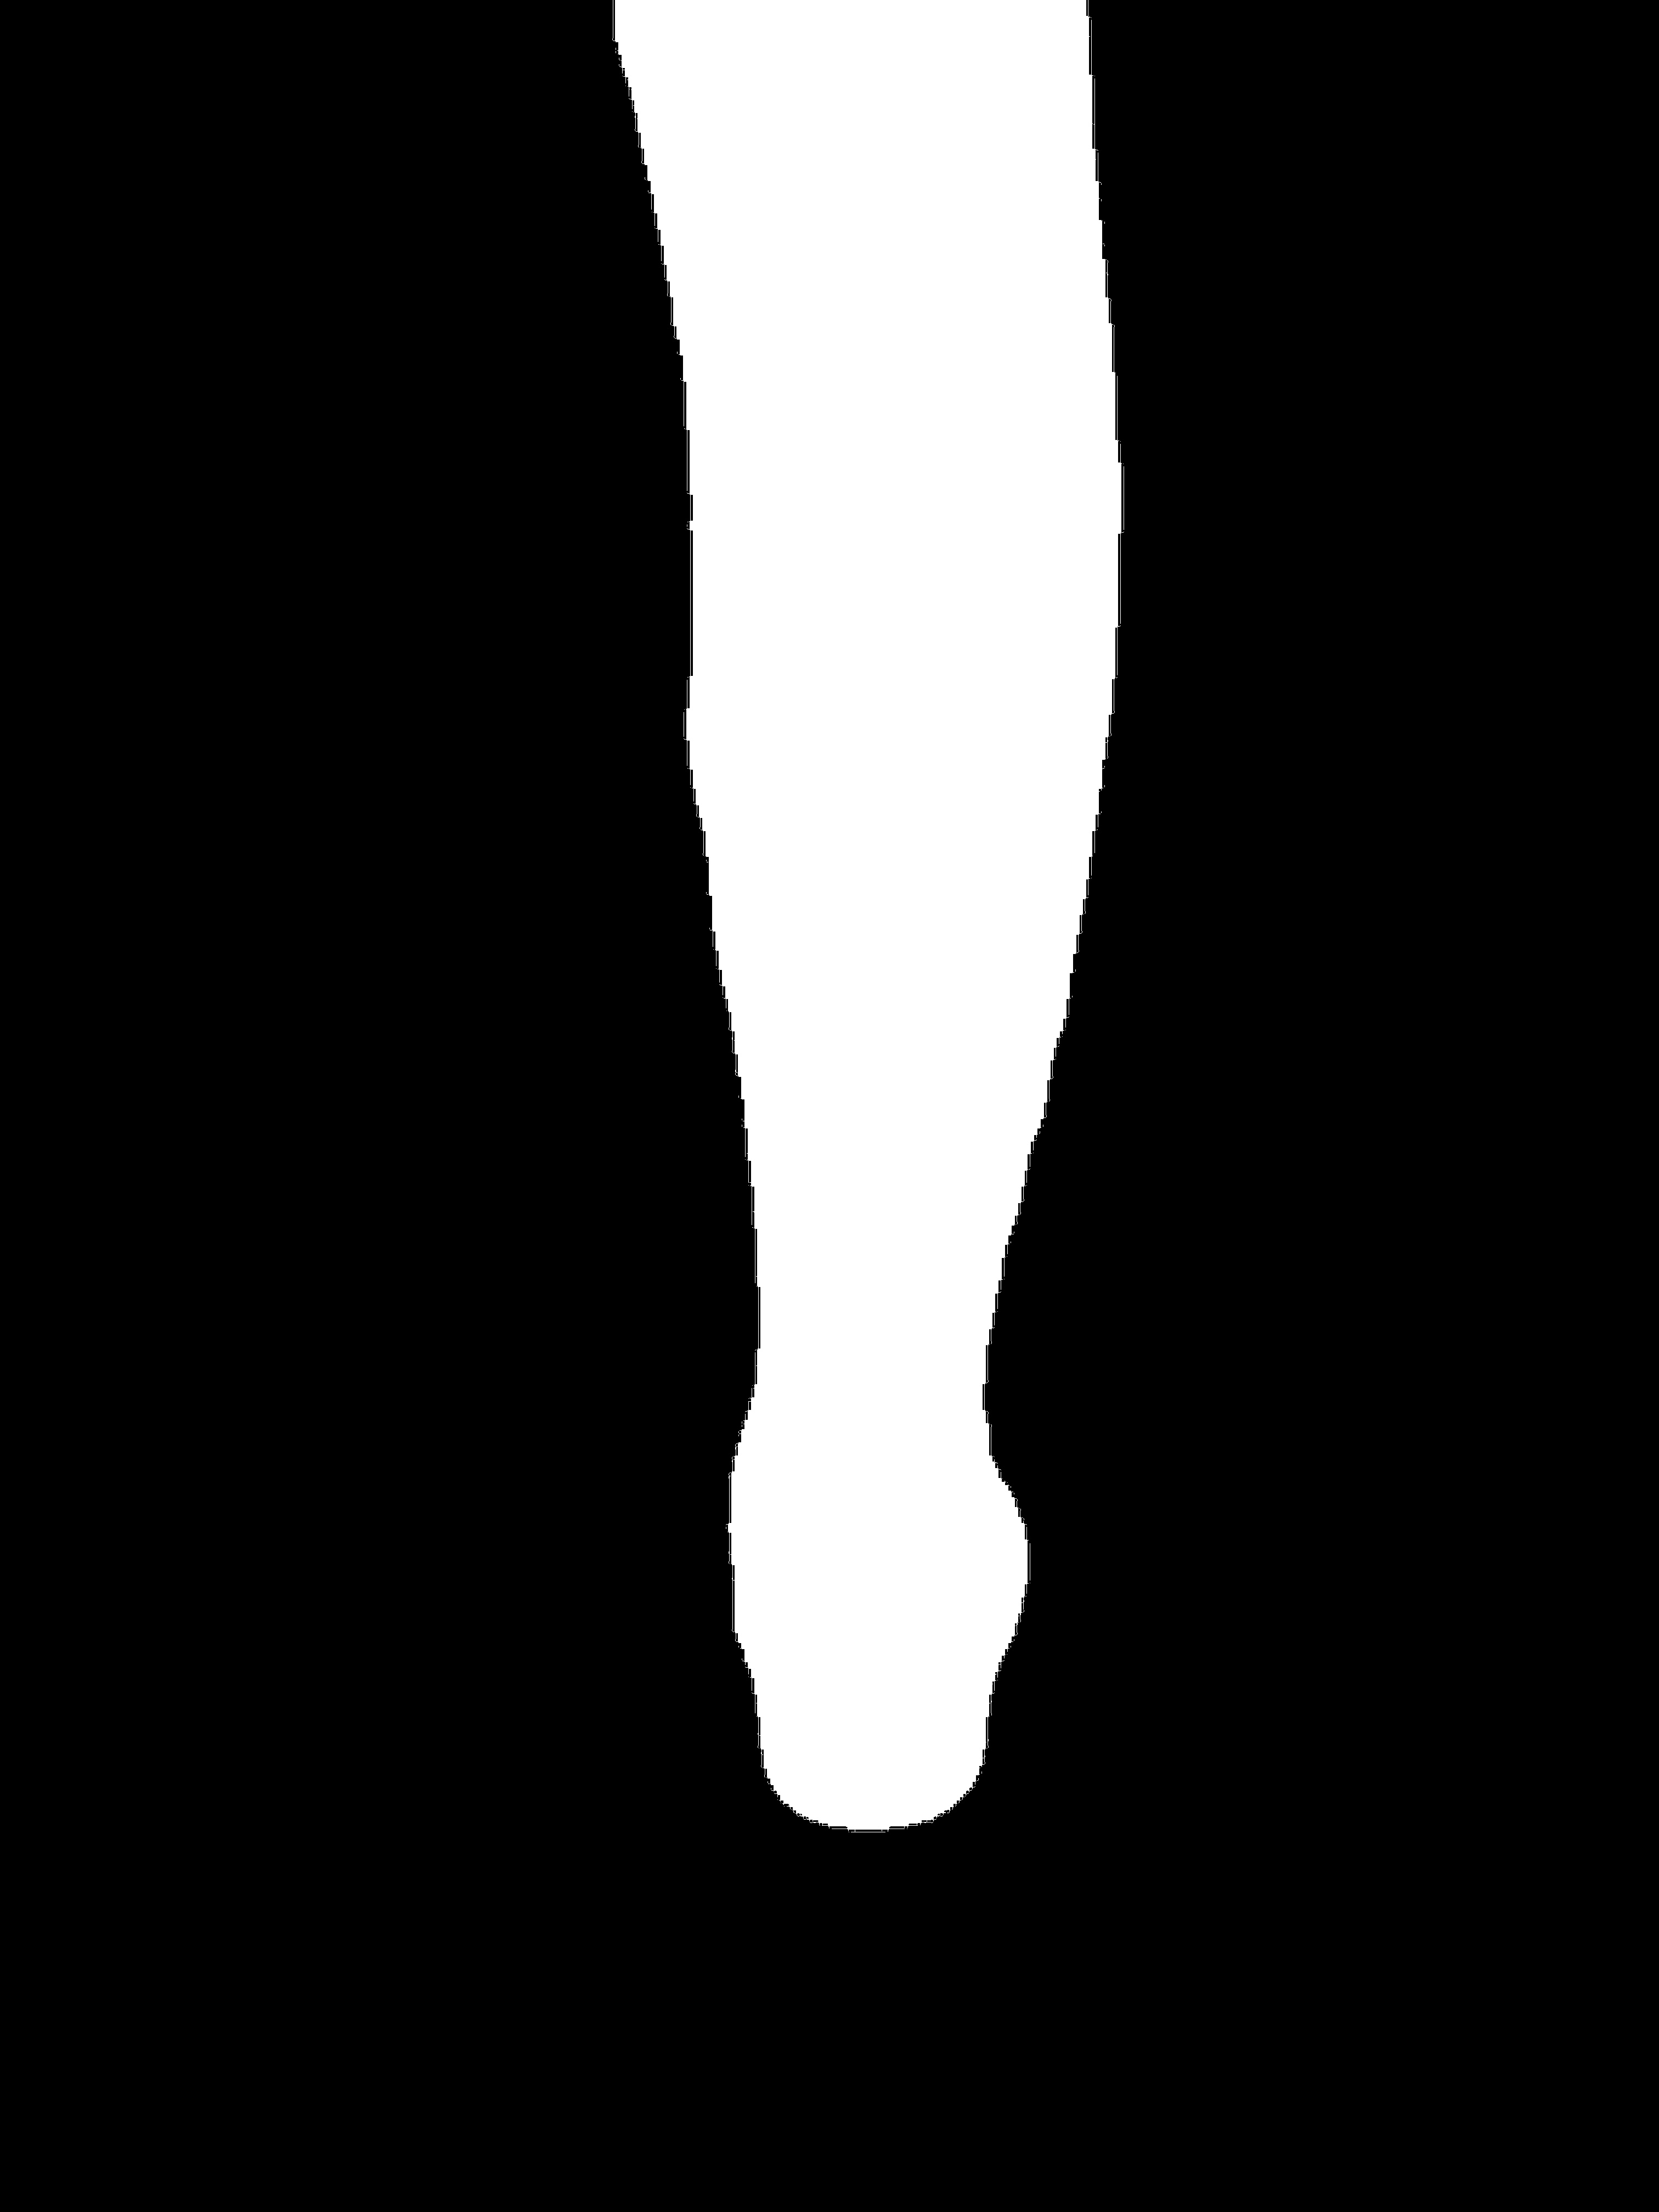
\includegraphics[width=.55\columnwidth]{KaanEksenMSc/figures/BatchProcessRioStudyII.jpeg}}
\caption{Region of interest results in study II}
\label{fig:BatchProcessRioStudyII}
\end{figure}

The batch process calculation is redesigned from the start. Initially, the image types are differentiated for processing the correct images with correct index types. Therefore, the foot side type (see Section \ref{sec:StudyIDatabase} for details) is used for differentiation in the scan file (i.e., image).

After the correct image selection, detecting the foot and leg is crucial. Therefore, deep learning algorithms are applied to extract the region of interest. Finally, DeepLabV3 is used based on the experiences obtained in Section \ref{sec:StudyIServicesAndBatchProcess} to detect the region of interest (see Figure \ref{fig:BatchProcessRioStudyII}).

Fallowing the region of interest detection, critical points are detected. There are four critical points in rearfoot angle calculation (see section for details \ref{sec:MethodologyFootDeformityDetection}). Each point requires specific points to be detected in the leg. In addition, each point is very close to the midpoint of the leg.

\begin{figure}[htbp]
\centering
\fbox{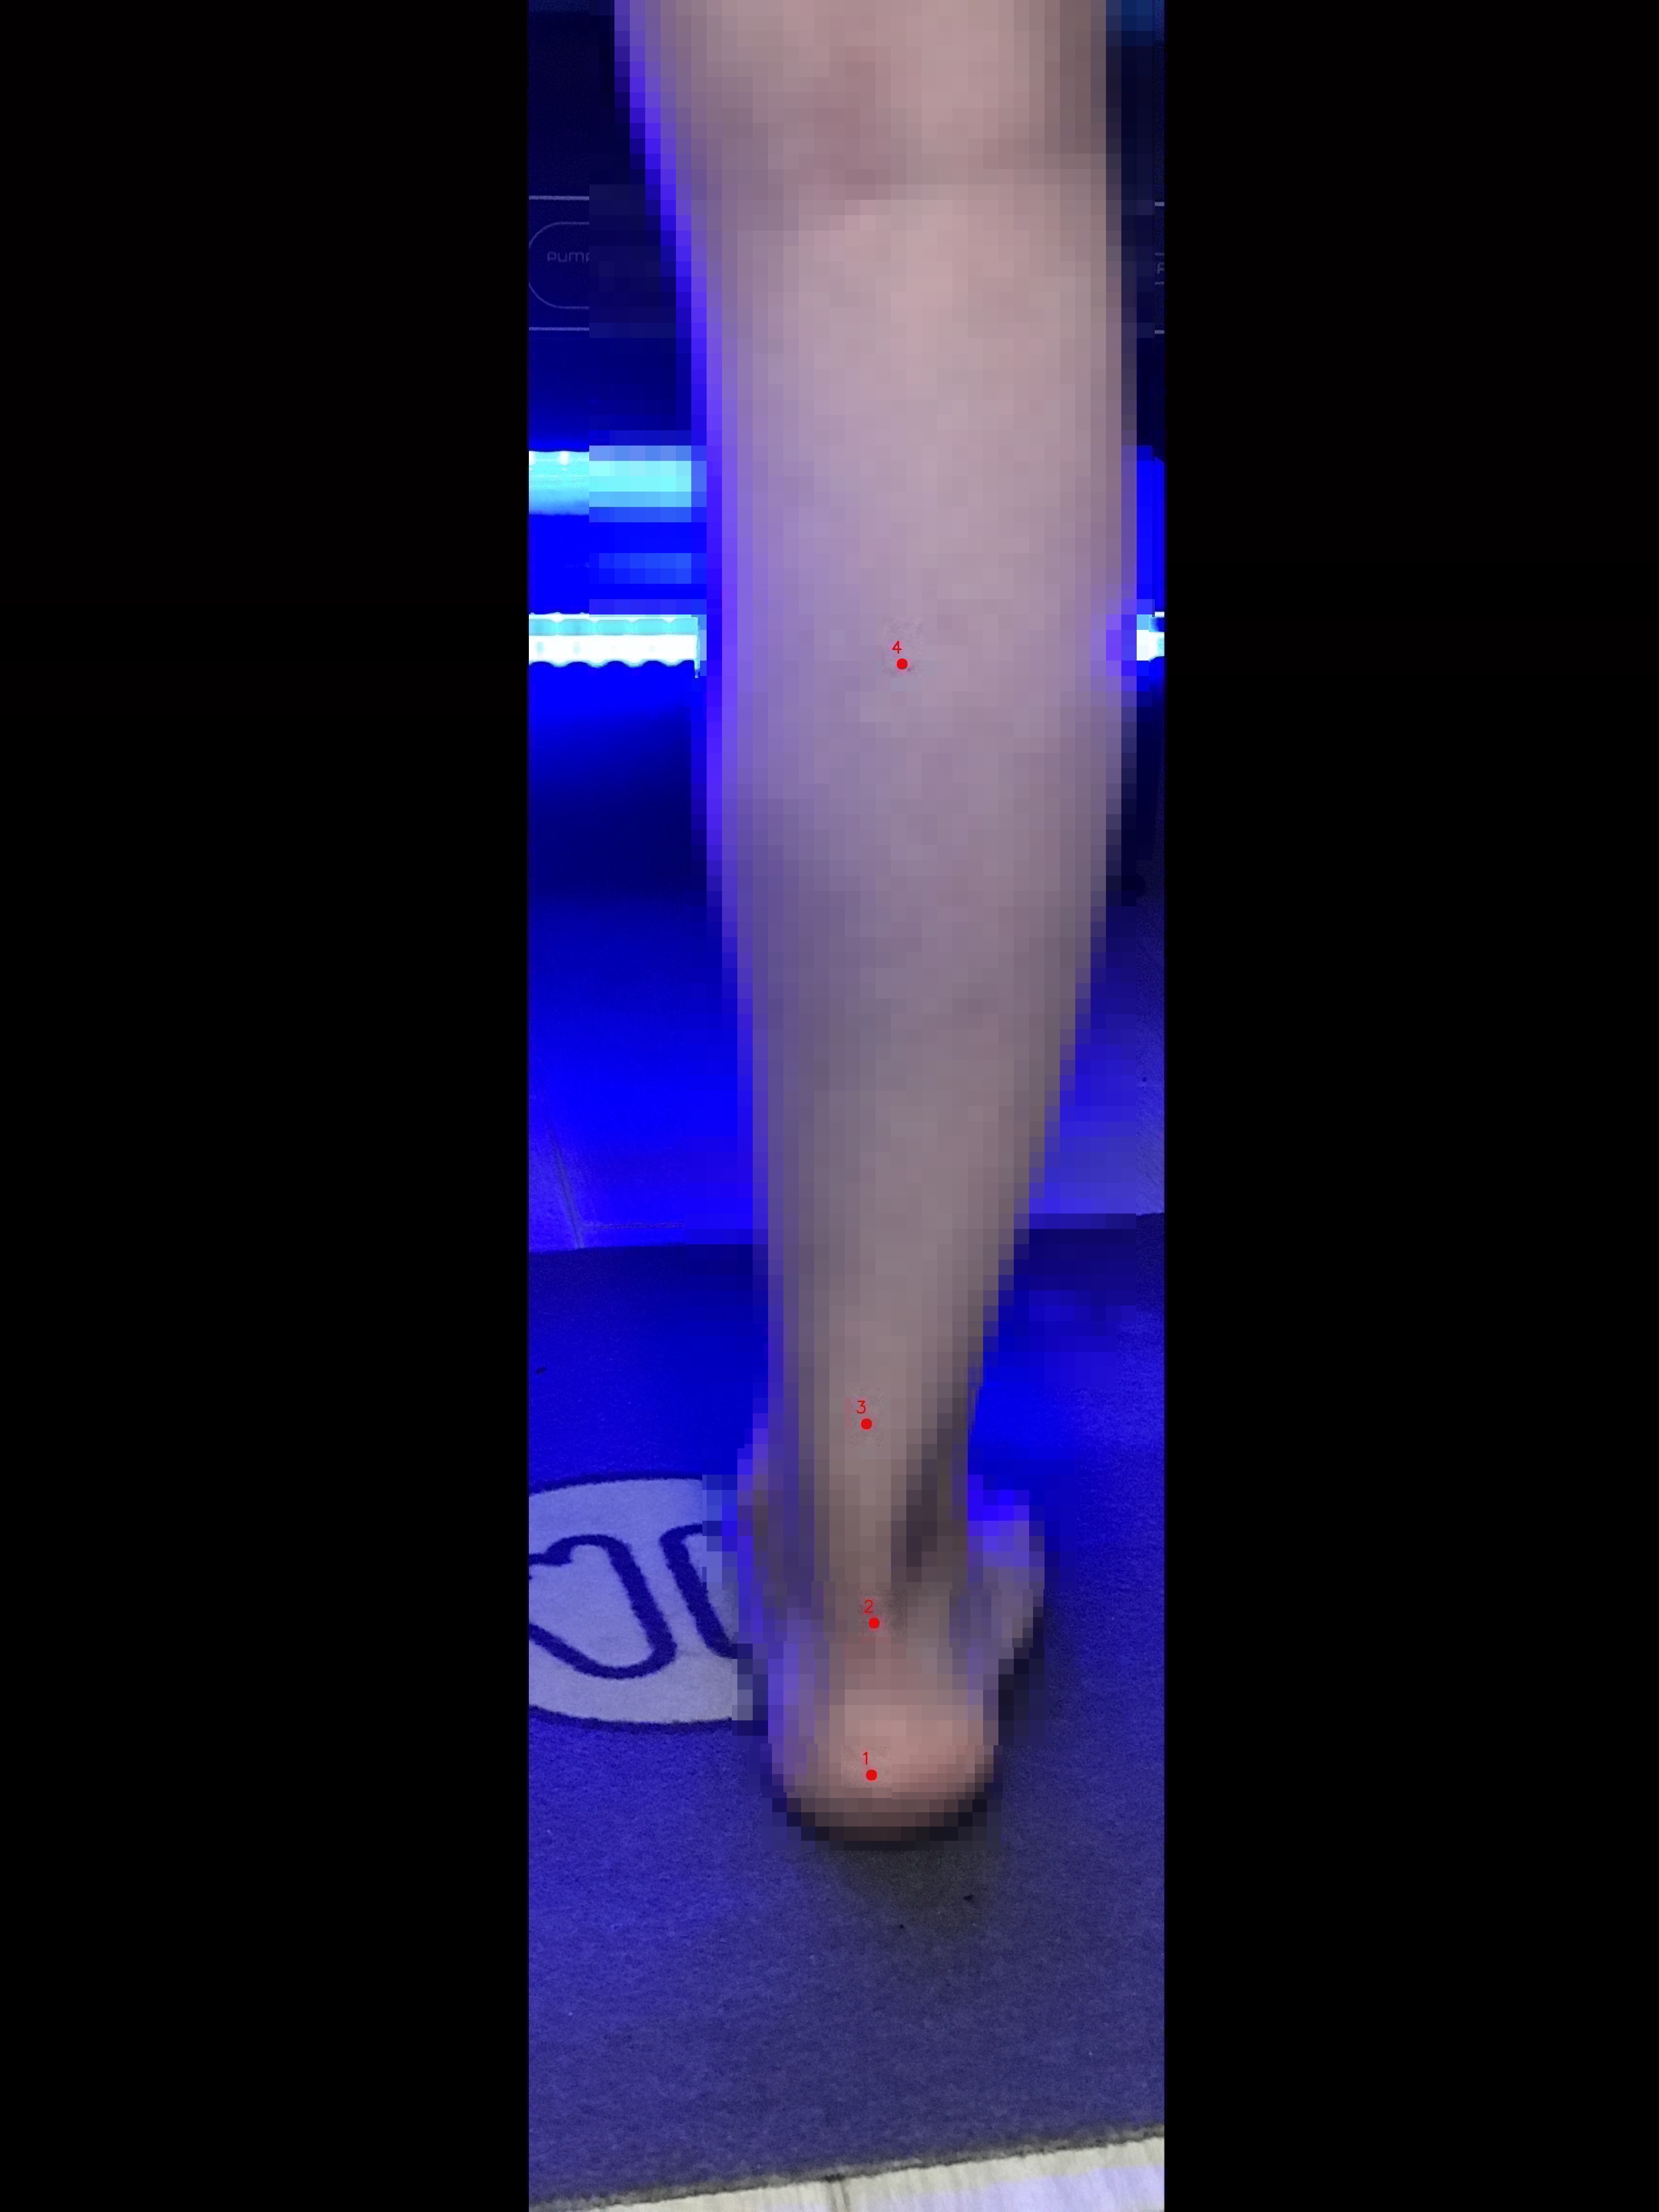
\includegraphics[width=.55\columnwidth]{KaanEksenMSc/figures/BatchProcessDotsStudyII.png}}
\caption{Calculated critical points for rearfoot angle (red dots)}
\label{fig:BatchProcessDotsStudyII}
\end{figure}

The first point base of the calcaneus is calculated based on the region of interest. Processing starts from the bottom of the image, where the initial region is detected wideness of the area is recorded. In case of the region of interest errors, the processing is continued until 30 percent of the image width from the initial region detection. If new wideness is more significant than 50 percent of the initial detection, new area wideness is considered the calcaneus's base.

The second point determination is based on the assumption that the ankle is the thinnest area in the leg. Therefore, the narrowing of the leg is sought, following the first point discovery. After this region is found, it is considered the second broken point, which is 5\% down by the region of interest. In addition, the third point has a similar discovery process. The only difference is that the third point is 5\% up by the region of interest

The fourth point corresponds to the narrowing point of the calf. Therefore, after the third point is found, narrowing is sought in the region.

\section{TEST AND EVALUATION}\label{sec:StudyIITestAndEvaluation}

This section will provide the test end evaluation process of the prototype system described in detail in previous sections. 

\begin{table}[htbp]
\begin{center}
\caption{Participant statistics in study II}
\vspace{23pt}
      \begin{tabular}{|c|c|c|c|c|} \hline
          & \textbf{Age} & \textbf{Weight} & \textbf{Height} & \textbf{BMI} \\ \hline
        \textbf{Avarage} & 22.67 & 70.89 & 173.11 & 23.24 \\ \hline
        \textbf{Max} & 29 & 100 & 190 & 30.19 \\ \hline
        \textbf{Min} & 21 & 50 & 159 & 19.05 \\ \hline
    \end{tabular}
\label{tab:StudyIIParticipantStatistics}
\end{center}
\end{table}

In the second study, the test data were collected through mobile applications though healthcare officials supervision. Therefore collected data were evaluated before the process. In addition, healthcare officials were provided with the how-to-use document, which explains how to use the application. 

The prototype was used by 9 participants, where 3 (33.33 \%) of them were female, and the remaining 6 (66,67 \%) were male, with an average age of 22.6 (see Table \ref{tab:StudyIParticipantStatistics} for details). Data is stored in online database which described in section \ref{sec:StudyIAnalysisAndDesign}. 

\begin{figure}[htbp]
\centering
\fbox{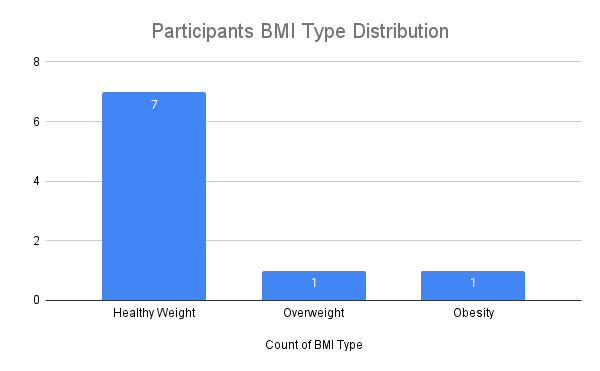
\includegraphics[width=.65\columnwidth]{KaanEksenMSc/figures/StudyIIParticipantsBMITypeDistribution.png}}
\caption{Participants BMI type distribution based on CDC in study II}
\label{fig:StudyIIParticipantsBMITypeDistribution}
\end{figure}

BMI is critical since most of the index calculations are based on the ratio to remove the effects of the weight. Population's average BMI is 23.2 (healthy weight), ( see Figure \ref{fig:StudyIIParticipantsBMITypeDistribution}). Therefore, this might not provide sufficient data for projection in different wight scales.

\begin{figure}[htbp]
\centering
\fbox{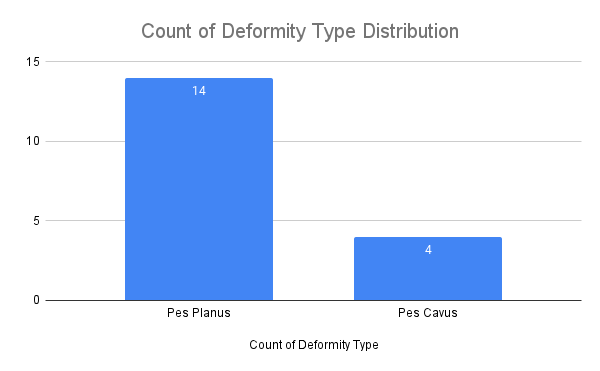
\includegraphics[width=.60\columnwidth]{KaanEksenMSc/figures/StudyIIFootDeformityTypeDistribution.png}}
\caption{Foot deformity type distribution in study II}
\label{fig:StudyIIFootDeformityTypeDistribution}
\end{figure} 

There were 18 foot photos out of 18 foot pictures for processing since all data were supervised. The healthcare specialists approved all the data provided to the system. Therefore participants' deformities are validated in the examination (see Figure  \ref{fig:StudyIIFootDeformityAutomatedDegreesAndDeformityResults}).

\begin{figure}[htbp]
\centering
\fbox{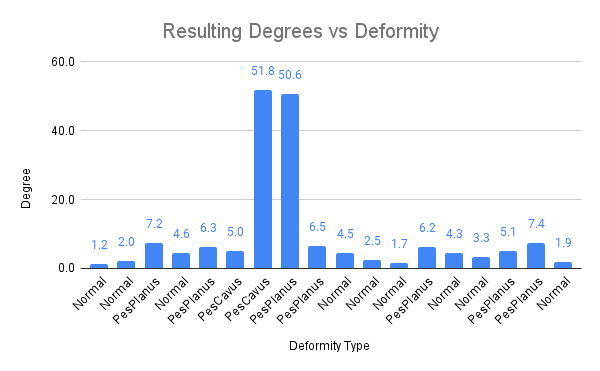
\includegraphics[width=.60\columnwidth]{KaanEksenMSc/figures/StudyIIFootDeformityAutomatedDegreesAndDeformityResults.png}}
\caption{Rear foot angle vs foot deformity in automated process results}
\label{fig:StudyIIFootDeformityAutomatedDegreesAndDeformityResults}
\end{figure} 

After the data collection, automated index calculations were conducted. Initial results showed that the findings of the healthcare officials and the system were 27,7\% matched. This low performance may be caused by multiple factors such as image angle, color disorientation, assumptions in point location determination. However, the primary factor is sensitivity to rear foot angle calculation error which was the angle between the two lines was limited to five degrees (see Figure \ref{fig:StudyIIFootDeformityAutomatedDegreesAndDeformityResults}). 
